\chapter{Spatial data}
\label{ch:spatial}

\begin{quotation}
  ``everything is related to everything else, but near things are more related than distant things.''
  \flushright{-- Waldo R. Tobler (1969)}
\end{quotation}

\textbf{Geostatistics} is a branch of statistics that deals explicitly
with data distributed in space and aims at explicitly modelling that
spatial relationship between the data. Originally developed in the
context of mining geology, the field has applications in petroleum
geology, environmental science, oceanography, hydrology, pedology,
ecology, epidemiology, and many more. In this chapter we will use an
environmental dataset to introduce some fundamental geostatistical
concepts:

\begin{center}
\begin{tabular}{c|cccc}
\#  & $x$    & $y$    & Zn & $z=\ln[\mbox{Zn}]$\\ \hline
1   & 181072 & 333611 & 1022 & 6.93 \\     
2   & 181025 & 333558 & 1141 & 7.04 \\
3   & 181165 & 333537 & 640  & 6.46 \\
$\vdots$ & $\vdots$ & $\vdots$ & $\vdots$ \\
50  & 180199 & 331591 & 375  & 5.93 \\
$\vdots$ & $\vdots$ & $\vdots$ & $\vdots$ \\
155 & 180627 & 330190 & 375  & 5.93 \\
\end{tabular}
\captionof{table}{ Locations and zinc concentrations of 155 samples of
  topsoil, collected in a flood plain of the river Meuse, near the
  village of Stein (Netherlands). $x$ and $y$ are the Easting and
  Northing (as metres), respectively, in Rijksdriehoek (RDH)
  (Netherlands topographical) map coordinates. The column labelled
  `Zn' contains the zinc concentration (in ppm) from composite samples
  of an area of approximately $15\times{15}$m.}
\label{tab:Meuse}
\end{center}

Now consider the position $\{x=179850,y=331650\}$ where no measurements
was taken. The question that this chapter addresses is: can we use the
surrounding data to estimate the Zn-concentration at this new
location? Or, bearing in mind the idiosyncrasies of compositional data
that were discussed in chapter~\ref{ch:compositional}: can we estimate
the logarithm of the Zr-concentration at this new location
($z$ in Table~\ref{tab:Meuse})?

\noindent\begin{minipage}[t][][b]{.55\textwidth}
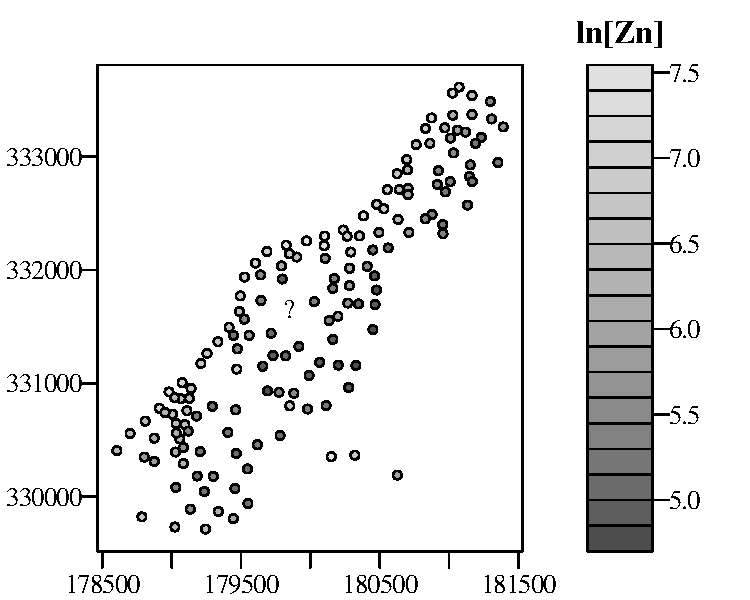
\includegraphics[width=\textwidth]{../figures/meusepoints.pdf}
\end{minipage}
\begin{minipage}[t][][t]{.45\textwidth}
  \captionof{figure}{Location map of the Meuse data. The question mark
    is located at a position $\{x=179850,y=331650\}$ where no
    measurements was taken. This chapter will use a geostatistical
    technique called \textbf{kriging} to estimate the (logarithm of)
    the zinc concentration at this location from the surrounding
    measurements.\\}
  \label{fig:meusepoints}
\end{minipage}

\section{The semivariogram}
\label{sec:semivariogram}

To assess the spatial correlation of the data, we begin by measuring
the inter-sample distances between the 155~samples in the Meuse
dataset:

\begin{center}
\begin{tabular}{c|cccccccccccc}
~  &  1 & 2 & 3 &  4  &  5  &  6  &  7  &  8  &  9 &  10 & $\ldots$ & 155 \\ \hline
1  &  0 &71 & 120 & 260 & 370 & 470 & 260 & 250 & 380 & 470 & $\ldots$ &3400 \\
2  &  ~ & 0 &140& 280 & 360 & 470 & 230 & 200 & 330 & 440 & $\ldots$ &3400 \\
3  &  ~ & ~ & 0 & 140 & 250 & 360 & 170 & 220 & 320 & 380 & $\ldots$ &3400 \\
4  &  ~ & ~ & ~ &  0  & 150 & 240 & 180 & 300 & 350 & 320 & $\ldots$ &3400 \\
5  &  ~ & ~ & ~ & ~   &  0  & 110 & 150 & 280 & 270 & 180 & $\ldots$ &3200 \\
6  &  ~ & ~ & ~ & ~   & ~   &  0 & 250 & 380 & 330 & 180 & $\ldots$ &3200 \\
7  &  ~ & ~ & ~ & ~   & ~   & ~  &  0 & 140 & 170 & 210 & $\ldots$ &3200 \\
8  &  ~ & ~ & ~ & ~   & ~   & ~  & ~  &  0  & 140 & 280 & $\ldots$ &3200 \\
9  &  ~ & ~ & ~ & ~   & ~   & ~  & ~  & ~   &  0  & 180 & $\ldots$ &3100 \\
10 &  ~ & ~ & ~ & ~   & ~   & ~  & ~  & ~   & ~   & 0   & $\ldots$ &3000 \\
$\vdots$ & ~   & ~ & ~ & ~ & ~ & ~ & ~ &
~ & ~   & ~ & $\ddots$ & $\vdots$ \\
155 & ~ & ~ & ~ & ~   & ~ & ~ & ~ & ~ & ~ & ~ & ~ & 0
\end{tabular}
\end{center}

\noindent where we show only the upper triangle because the lower
triangle contains exactly the same values. Next, we compute the
differences between the Zn-concentations of the samples, thus
producing a second $155\times{155}$ matrix:

\begin{center}
\begin{tabular}{c|cccccccccccc}
~ & 1 & 2 & 3 & 4 & 5 & 6 & 7 & 8 & 9 & 10& $\ldots$ & 155\\ \hline
1 & 0 & ~ & ~ & ~ & ~ & ~ & ~ & ~ & ~ & ~ & ~ & ~ \\
2 & 0.16 & 0 & ~ & ~ & ~ & ~ & ~ & ~ & ~ & ~ & ~ & ~ \\
3 & 0.66 & 0.82 & 0 & ~ & ~ & ~ & ~ & ~ & ~ & ~ & ~ & ~ \\
4 & 2.0 & 2.1 & 1.3 & 0 & ~ & ~ & ~ & ~ & ~ & ~ & ~ & ~ \\
5 & 1.9 & 2.0 & 1.2 & 0.065 & 0 & ~ & ~ & ~ & ~ & ~ & ~ & ~ \\
6 & 1.8 & 2.0 & 1.2 & 0.13 & 0.062 & 0 & ~ & ~ & ~ & ~ & ~ & ~ \\
7 & 1.5 & 1.7 & 0.87 & 0.42 & 0.36 & 0.29 & 0 & ~ & ~ & ~ & ~ & ~ \\
8 & 1.3 & 1.5 & 0.64 & 0.65 & 0.58 & 0.52 & 0.23 & 0 & ~ & ~ & ~ & ~ \\
9 & 1.5 & 1.7 & 0.87 & 0.42 & 0.36 & 0.30 & 0.0041 & 0.22 & 0 & ~ & ~ & ~ \\
10& 2.4 & 2.6 & 1.8  & 0.48 & 0.54 & 0.61 & 0.90 & 1.1 & 0.90 & 0 & ~ & ~ \\
$\vdots$ & $\vdots$ & $\vdots$ & $\vdots$ & $\vdots$ & $\vdots$ &
$\vdots$ & $\vdots$ & $\vdots$ & $\vdots$ & $\vdots$ & $\ddots$ & ~ \\
155 & 1.4 & 1.6 & 0.76 & 0.53 & 0.47 & 0.41 & 0.11 & 0.11 & 0.11 & 1.0 & $\ldots$ & 0\\
\end{tabular}
\end{center}

\noindent where we show only the lower triangle because the upper
triangle contains exactly the same values. We can then merge the two
tables and select all the pairs of samples that are within a distance
of 150~m from each other:

\begin{center}
\begin{tabular}{@{}c@{~~}|@{~~}c@{~~}c@{~~}c@{~~}c@{~~}c@{~~}c@{~~}c@{~~}c@{~~}c@{~~}c@{~~}c@{~~}c@{}}
~ &  1 & 2 & 3 &  4  &  5  &  6  &  7  &  8  &  9 &  10 & $\ldots$ & 155 \\ \hline
1 &  0 & \boxed{71} & \boxed{120} & 260 & 370 & 470 & 260 & 250 & 380 & 470 & $\ldots$ & 3400 \\
2 & \boxed{0.16} & 0 & \boxed{140} & 280 & 360 & 470 & 230 & 200 & 330 & 440 & $\ldots$ & 3400 \\
3 & \boxed{0.66} & \boxed{0.82} & 0 & \boxed{140} & 250 & 360 & {170} & 220 & 320 & 380 & $\ldots$ & 3400 \\
4 & 2.0 & 2.1 & \boxed{1.3} & 0 & \boxed{150} & 240 & 180 & 300 & 350 & 320 & $\ldots$ & 3400 \\
5 & 1.9 & 2.0 & 1.2 & \boxed{0.065} & 0  & \boxed{110} & \boxed{150} & 280 & 270 & {180} & $\ldots$ & 3200 \\
6 & 1.8 & 2.0 & 1.2 & 0.13 & \boxed{0.062} & 0 & 250 & 380 & 330 & {180} & $\ldots$ & 3200 \\
7 & 1.5 & 1.7 & 0.87 & 0.42 & \boxed{0.36} & 0.29 & 0 & \boxed{140} & {170} & 210 & $\ldots$ & 3200 \\
8 & 1.3 & 1.5 & 0.64 & 0.65 & 0.58 & 0.52 & \boxed{0.23} & 0  & \boxed{140} & 280 & $\ldots$ & 3200 \\
9 & 1.5 & 1.7 & 0.87 & 0.42 & 0.36 & 0.30 & 0.0041 & \boxed{0.22} & 0 & {180} & $\ldots$ & 3100 \\
10& 2.4 & 2.6 & 1.8 & 0.48 & 0.54 & 0.61 & 0.90 & 1.1 & 0.90 & 0 & $\ldots$ & 3000 \\
$\vdots$ & $\vdots$ & $\vdots$ & $\vdots$ & $\vdots$ & $\vdots$ &
$\vdots$ & $\vdots$ & $\vdots$ & $\vdots$ & $\vdots$ & $\ddots$ & $\vdots$ \\
155 & 1.4 & 1.6 & 0.76 & 0.53 & 0.47 & 0.41 & 0.11 & 0.11 & 0.11 & 1.0 & $\ldots$ & 0 \\
\end{tabular}
\captionof{table}{Composite data table with the inter-sample distances
  above the diagonal and the log-contrasts of the corresponding
  zinc-concentrations below the diagonal. Boxed values mark sample
  pairs that are located within 150 metres of each other.}
\label{tab:h=100}
\end{center}

\noindent we can then use the boxed values below the diagonal to
define the sample \textbf{semivariance} as:

\begin{equation}
\gamma[h] = \sum\limits_{k}^{n(h)}\frac{(z_{i[k]}-z_{j[k]})^2}{2 n(h)}
\end{equation}

\noindent where $n(h)$ is the number of sample pairs that fall within
a distance (or `lag') $h$ of each other, and $\{z_{i[k]},z_{j[k]}\}$
are the $\log_{10}$(Zn) values for the $k$\textsuperscript{th} sample
pair.  For the data shown in Table~\ref{tab:h=100}, there are 166
sample pairs that fall within a distance of 150~m of each other (of
which only 9 are shown due to space constraints), and the sample
semivariance equals:

\[
\gamma[0<h\leq{150}] =
\frac{0.16^2 + 0.66^2 + 0.82^2 + \ldots}{2 \times 166} = 0.10
\]

We can repeat this calculation for all sample pairs that are within a
distance of 150 to 300 metres of each other:

\begin{center}
\begin{tabular}{@{}c@{~~}|@{~~}c@{~~}c@{~~}c@{~~}c@{~~}c@{~~}c@{~~}c@{~~}c@{~~}c@{~~}c@{~~}c@{~~}c@{}}
~  &  1 & 2 & 3 &  4  &  5  &  6  &  7  &  8  &  9 &  10 & $\ldots$ & 155 \\ \hline
1  &  0 & 71 & 120 & \boxed{260} & {370} & 470 & \boxed{260} & \boxed{250} & 380 & 470 & $\ldots$ & 3400 \\
2 & 0.16 & 0 & 140 & \boxed{280} & {360} & 470 & \boxed{230} & \boxed{200} & {330} & 440 & $\ldots$ & 3400 \\
3 & 0.66 & 0.82 & 0 & 140 & \boxed{250} & {360} & \boxed{170} & \boxed{220} & {320} & {380} & $\ldots$ & 3400 \\
4 & \boxed{2.0} & \boxed{2.1} & 1.3  & 0 & 150 & \boxed{240} & \boxed{180} & \boxed{300} & {350} & {320} & $\ldots$ & 3400 \\
5 & 1.9 & 2.0 & \boxed{1.2} & 0.065 & 0 & 110 & 150 & \boxed{280} & \boxed{270} & \boxed{180} & $\ldots$ & 3200 \\
6 & 1.8 & 2.0 & 1.2 & \boxed{0.13} & 0.062 & 0 & \boxed{250} & {380} & {330} & \boxed{180} & $\ldots$ & 3200 \\
7 & \boxed{1.5} & \boxed{1.7} & \boxed{0.87} & \boxed{0.42} & 0.36 & \boxed{0.29} & 0 & 140 & \boxed{170} & \boxed{210} & $\ldots$ & 3200 \\
8 & \boxed{1.3} & \boxed{1.5} & \boxed{0.64} & \boxed{0.65} & \boxed{0.58} & 0.52 & 0.23 & 0  & 140 & \boxed{280} & $\ldots$ & 3200 \\
9 & 1.5 & 1.7 & 0.87 & 0.42 & \boxed{0.36} & 0.30 & \boxed{0.0041} & 0.22 & 0 & \boxed{180} & $\ldots$ & 3100 \\
10 & 2.4 & 2.6 & 1.8 & 0.48 & \boxed{0.54} & \boxed{0.61} & \boxed{0.90} & \boxed{1.1} & \boxed{0.90} & 0 & $\ldots$ & 3000 \\
$\vdots$ & $\vdots$ & $\vdots$ & $\vdots$ & $\vdots$ & $\vdots$ &
$\vdots$ & $\vdots$ & $\vdots$ & $\vdots$ & $\vdots$ & $\ddots$ & $\vdots$ \\
155 & 1.4 & 1.6 & 0.76 & 0.53 & 0.47 & 0.41 & 0.11 & 0.11 & 0.11 & 1.0 & $\ldots$ & 0 \\
\end{tabular}
\captionof{table}{Boxed values mark inter-sample distances of 150 to
  300 metres (above the diagonal) and their corresponding log-contrast
  (below the diagonal).}
\label{tab:h=300}
\end{center}

There are 530 sample pairs that fall within a 150--300~m distance of
each other, resulting in a semivariance of:

\[
\gamma[150<h\leq{300}] =
\frac{2.0^2 + 1.5^2 + 1.3^2 + 2.1^2 + \ldots}{2 \times 530} = 0.28
\]

\noindent which is greater than $\gamma[0<h\leq{150}]$. Continuing
these calculations for progressively increasing values of $h$ produces
an empirical \textbf{semivariogram}:

\noindent\begin{minipage}[t][][b]{.3\textwidth}
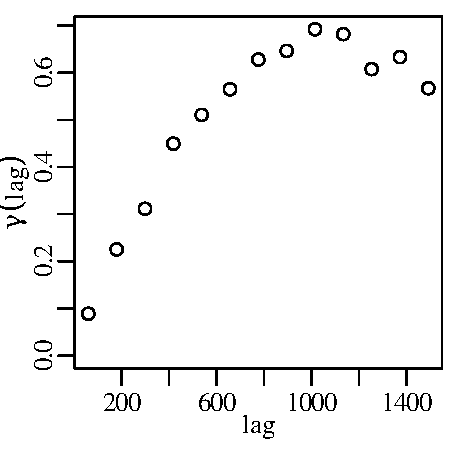
\includegraphics[width=\textwidth]{../figures/semivariogram.pdf}
\end{minipage}
\begin{minipage}[t][][t]{.7\textwidth}
  \captionof{figure}{Empirical semivariogram of the Meuse data. The
    semivariance is low at first and then gradually rises with
    increasing lag before levelling off to a plateau. Because the
    semivariance is inversely proportional to the degree of spatial
    correlation, the semivariogram tells us that there is relatively
    little variability among samples that are located close together,
    and more variability among samples that are far apart.  In other
    words, the semivariogram formalises Waldo's \textit{First Law of
      Geography}, which was quoted at the beginning of this chapter.}
  \label{fig:semivariogram}
\end{minipage}

\section{Semivariogram models}
\label{sec:semivariogram-models}

Now that we have quantified the degree of spatial variability or,
equivalently, the degree of spatial correlation, the next step in the
kriging method is to parameterise the semivariogram. There are several
equations to do this, such as the exponential model:

\begin{equation}
  \gamma[h] = c_s + (c_n-c_s) \exp\left[-\frac{h}{c_r}\right]
  \label{eq:semivariogramexponential}
\end{equation}

\noindent the Gaussian model:

\begin{equation}
  \gamma[h] = c_s + (c_n-c_s) \exp\left[-\frac{h^2}{c_r^2}\right]
  \label{eq:semivariogramgaussian}
\end{equation}

\noindent the linear model:

\begin{equation}
  \left\{
  \begin{aligned}
  \gamma[h] = & c_n + \frac{(c_s-c_n) h}{c_r} & \mbox{~if~}{h}\leq{c_r}\\
    \gamma[h] = & c_s & \mbox{~if~} h>c_r 
  \end{aligned}
  \right.
    \label{eq:semivariogramlinear}
\end{equation}

\noindent and the spherical model:

\begin{equation}
  \left\{
  \begin{aligned}
    \gamma[h] = & c_n + (c_s-c_n)
    \left(\frac{3}{2}\frac{h}{c_r} -
    \frac{1}{2}\left[\frac{h}{c_r}\right]^3\right)
    & \mbox{~if~}{h}\leq{c_r}\\
    \gamma[h] = & c_s & \mbox{~if~} h>c_r
  \end{aligned}
  \right.
  \label{eq:semivariogramspherical}
\end{equation}

\noindent
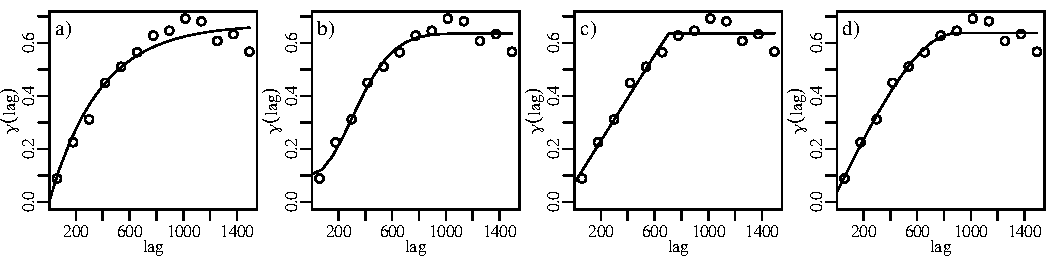
\includegraphics[width=\textwidth]{../figures/semivariogramfit.pdf}
\begingroup \captionof{figure}{Parametric semivariogram fits for the
  Meuse data, using the a) Gaussian, b) exponential, c) linear and d)
  spherical models.\\}
\label{fig:semivariogramfit}
\endgroup

Equations~\ref{eq:semivariogramexponential}--\ref{eq:semivariogramspherical}
contain three parameters:

\begin{enumerate}
\item The \textbf{range} ($c_r$) is the distance within which samples
  are spatially correlated, and beyond which they are independent from
  each other.

\item The \textbf{sill} ($c_s$) quantifies the long range background
  variability of the the data.\\

\item The \textbf{nugget} ($c_n$) is the excess variance at zero
  distance. In principle samples that are co-located should have the
  same value, but in practice this is not always the case and the
  semivariogram may have a non-zero intercept. This \textit{nugget
    effect} may be caused by measurement errors, or it may be caused
  by features occurring at scales smaller than the sample.
\end{enumerate}

\noindent\begin{minipage}[t][][b]{.35\textwidth}
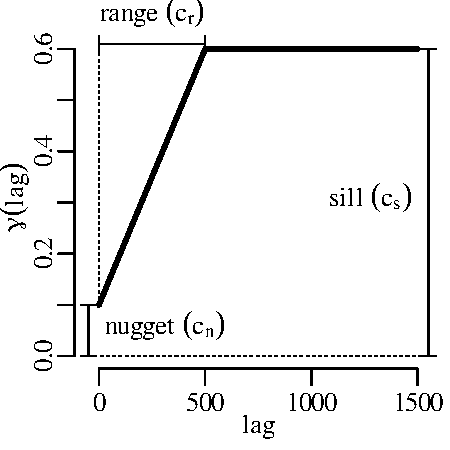
\includegraphics[width=\textwidth]{../figures/snr.pdf}
\end{minipage}
\begin{minipage}[t][][t]{.65\textwidth}
  \captionof{figure}{Illustration of the range, sill and nugget of a
    generic linear semivariogram model. The same three parameters also
    control the shape of the exponential, Gaussian and spherical
    models. In the case of the Meuse dataset, the nugget effect is
    likely caused by the fact that the zinc concentrations were
    averaged over a 15$\times$15~metre area, and that the variability
    within this sampling area is not captured by the semivariogram.}
  \label{fig:snr}
\end{minipage}

\section{Kriging interpolation}
\label{sec:kriging}

The kriging method is named after the South Afrian mining geologist
Danie Gerhardus Krige, who laid the foundations for the method in his
Master's thesis.  Given the best analytical fit to the semivariogram,
the kriging algorithm interpolates the data between the measurements
as follows:

\begin{equation}
z(x_\circ,y_\circ) = \sum\limits_{i=1}^n w_i z(x_i,y_i)
\label{eq:kriging}
\end{equation}

\noindent where, for the Meuse dataset, $z(x,y)$ is the zinc
concentration at some location $\{x,y\}$; $\{x_i,y_i\}$ are the
coordinates of the $i$\textsuperscript{th} site (out of $n$); and
$\{x_\circ,y_\circ\}$ is the location of a the new site for which we
want to estimate the zinc concentration. $w_i$ is a weighting
parameter that depends on the distance between locations $\{x_i,y_i\}$
and $\{x_\circ,y_\circ\}$ and on the spatial correlation at that
distance, which is captured by the analytical fit to the
semivariogram. The weights can be estimated with the following matrix
expression:

\begin{equation}
  \left[
    \begin{array}{@{}c@{}}
      w_1 \\
      w_2 \\
      \vdots \\
      w_n \\
      \lambda
    \end{array}
    \right]
  =
  \left[
    \begin{array}{cccccc}
      c_n & \gamma[h_{1,2}] & \gamma[h_{1,3}] & \ldots & \gamma[h_{1,n}] & 1 \\
      \gamma[h_{2,1}] & c_n & \gamma[h_{2,3}] & \ldots & \gamma[h_{2,n}] & 1 \\
      \vdots & \vdots & \vdots & \ddots & \vdots \\
      \gamma[h_{n,1}] & \gamma[h_{n,2}] & \gamma[h_{n,3}] & \ldots & c_n & 1 \\
      1 & 1 & 1 & \ldots & 1 & 0 \\
    \end{array}
    \right]^{-1}
  \left[
    \begin{array}{c}
      \gamma[h_{1,\circ}] \\
      \gamma[h_{2,\circ}] \\
      \vdots \\
      \gamma[h_{n,\circ}]\\
      1
    \end{array}
    \right]
\label{eq:krigingweights}
\end{equation}

\noindent where $\lambda$ is a \textit{Lagrange multiplier} that is
used to ensure that the weights add up to one; and $h_{i,j}$ is the
distance between points $i$ and $j$:

\begin{equation}
h_{i,j} = \sqrt{(x_i-x_j)^2 + (y_i-y_j)^2}
\end{equation}

Fitting a spherical variogram to the Meuse dataset yields a nugget
$c_n = 0.035$, a sill $c_s = 0.64$ and a range of $c_r =
892$~metres. Fitting a kriging model to location
$\{x_\circ=179850,y_\circ=331650\}$ of Figure~\ref{fig:meusepoints}
then yields the following results:

\begin{equation}
  \left[
    \begin{array}{@{}c@{}}
      w_1 \\
      w_2 \\
      w_3 \\
      \vdots\\
      w_{50}\\
      \vdots\\
      w_{155} \\
      \lambda
    \end{array}
    \right]
  =
  \left[
    \begin{array}{@{}c@{}}
      0.0022 \\
      -0.00030 \\
      0.00022 \\
      \vdots \\
      -0.028 \\
      \vdots \\
      0.0019 \\
      0.0015
    \end{array}
    \right]
  =
  \left[
    \begin{array}{c@{}c@{~}c@{~}c@{~}c@{~}c@{~}c@{~}c@{}}
      0.035 & 0.11  & 0.15  & \ldots & 0.64   & \ldots & 0.64   & 1 \\
      0.11  & 0.035 & 0.18  & \ldots & 0.64   & \ldots & 0.64   & 1 \\
      0.15  & 0.18  & 0.035 & \ldots & 0.64   & \ldots & 0.64   & 1 \\
      \vdots & \vdots & \vdots & \ddots & \vdots & \ddots & \vdots & \vdots \\
      0.64   & 0.64   & 0.64   & \ldots & 0.035 & \ldots & 0.64   & 1 \\
      \vdots & \vdots & \vdots & \ddots & \vdots & \ddots & \vdots & \vdots \\
      0.64   & 0.64   & 0.64   & \ldots & 0.64   & \ldots & 0.035 & 1 \\
      1      & 1      & 1      & \ldots & 1      & \ldots & 1      & 0 \\
    \end{array}
    \right]^{-1}
  \left[
    \begin{array}{@{}c@{}}
      0.64 \\
      0.64 \\
      0.64 \\
      \vdots \\
      0.37 \\
      \vdots \\
      0.64 \\
      1
    \end{array}
    \right]
\end{equation}

\noindent in which we can recognise the nugget ($c_s = 0.035$) and the
sill ($c_s = 0.64$) for all the sample pairs that are separated by a
distance of zero or more than $c_r = 892$~metres, respectively.  Given
the 155 zinc (logged) concentration measurements of
Table~\ref{tab:Meuse}, the logged zinc concentration of location
$\{x_\circ=179850,y_\circ=331650\}$ is given by

\[
z_{x_\circ,y_\circ} = 0.0022 \times 6.93 - 0.00030 \times 7.04 +
0.00022 \times 6.46 + \ldots - 0.028 \times 5.93 + \ldots +
0.0019 \times 5.93 = 4.96
\]

\noindent corrsponding to a zinc concentration of $\exp[4.96]$ =
143~ppm. Repeating the same exercise for a grid of points spanning the
entire sampling area:

\noindent\begin{minipage}[t][][b]{.6\textwidth}
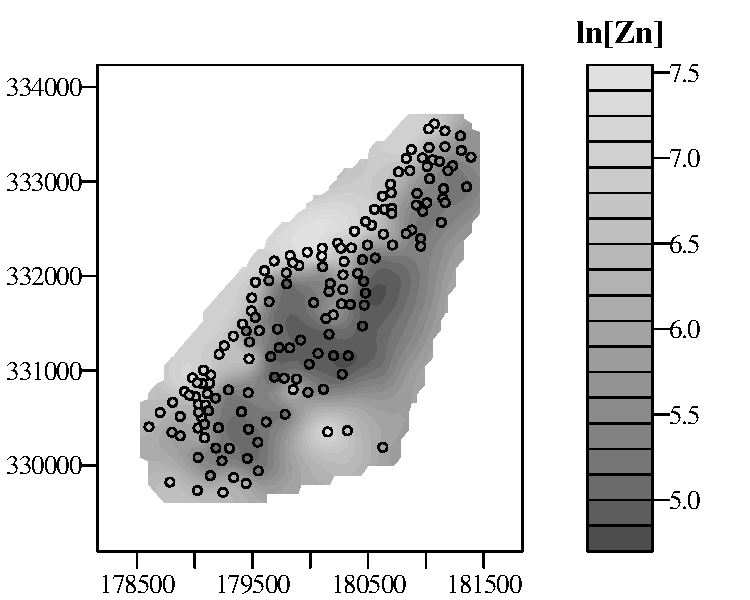
\includegraphics[width=\textwidth]{../figures/meusecontour.pdf}
\end{minipage}
\begin{minipage}[t][][t]{.39\textwidth}
  \captionof{figure}{
    The kriging interpolation results for the Meuse
    dataset shown as a filled contour plot, with the measurements of
    Figure~\ref{fig:meusepoints} added as points of comparison. The
    extent of the contour plot is limited to immediate vicinity of the
    measurements because kriging is an interpolation method and
    \emph{not} an \emph{extrapolation} method.\\
  }
  \label{fig:meusecontour}
\end{minipage}

The uncertainty (variance) of the kriging estimate is given by

\begin{equation}
  s^2(x_\circ,y_\circ) = \lambda + \sum\limits_{i=1}^n \gamma[h_{i,\circ}] w_i
  \label{eq:kriginvar}
\end{equation}

\noindent where $\lambda$ is the Lagrange multiplier of
Equation~\ref{eq:krigingweights}. For location
$\{x_\circ=179850,y_\circ=331650\}$:

\[
s^2(x_\circ,y_\circ) = 0.00029 + 0.64 \times 0.0022 - 0.64 \times
0.00030 + \ldots = 0.21
\]

Using the error propagation formula for the natural logarithm
(Equation~\ref{eq:logarithms}), this tells us the relative uncertainty
(i.e. the coefficient of variation) of the new measurement is
$s[z]/z=\sqrt{0.21}=46$\%. Repeating this exercise for the entire grid
of $\{x,y\}$-values:

\noindent\begin{minipage}[t][][b]{.6\textwidth}
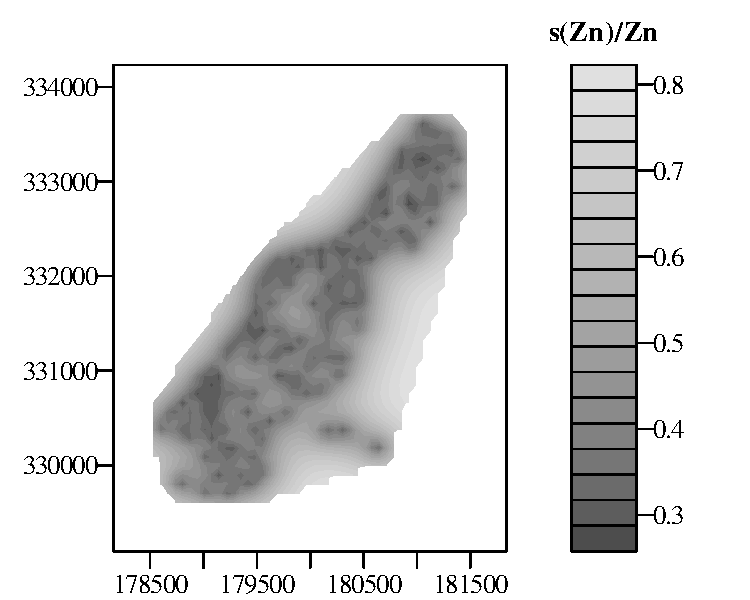
\includegraphics[width=\textwidth]{../figures/meusecontourerr.pdf}\\
\end{minipage}
\begin{minipage}[t][][t]{.39\textwidth}
  \captionof{figure}{ Contour plot of the relative uncertainty
    (coefficient of variation) of the kriging interpolation estimates
    of Figure~\ref{fig:meusecontour}. Note how the uncertainties are
    the greatest near the edges of the dataset, confirming again that
    kriging is not an extrapolation but an interpolation method.\\ }
  \label{fig:meusecontourerr}
\end{minipage}

This particular algorithm is known as \textbf{ordinary kriging}.
Other, more sophisticated variants of the kriging method exist that
relax some of the simplifying assumptions that are made by the
ordinary kriging.  For example:

\begin{enumerate}
\item Ordinary kriging assumes that the data is \textbf{stationary},
  and has a constant mean and variance. Minor violations of this
  assumption can be corrected by detrending the data.
\item The semivariogram models of
  Section~\ref{sec:semivariogram-models} assumed that the spatial
  correlation was \textbf{isotropic}. This means that the semivariance
  was only a function of the lag and not of the direction. This
  assumption may not always be appropriate. For example, valleys in a
  fold-and-thrust belt may be preferentially oriented in a particular
  direction. To accommodate these situations, anisotropic
  semivariogram models can be created that require additional
  parameters.
\item Using Equation~\ref{eq:kriging}, the kriging interpolation for a
  new location involved the values of all $n$ measurements.  This is
  fine for the relatively small Meuse dataset ($n=155)$, but for much
  larger datasets, the matrix inversion of
  Equation~\ref{eq:krigingweights} becomes computationally too
  demanding.  This problem can be solved by using only measurements
  that are reasonably close to the new sample for the interpolation.
\end{enumerate}

